\section{INTRODUCTION}

Energy efficiency is the ratio of useful work performed over the total energy supplied to a conversion process or device. 
Increasing energy efficiency is a current need of society because it reduces energy production demand to perform the same work~\citep{report:iea_efficiency}. 
This reduction has economic and environmental benefits, such as reducing vehicles’ cost of use and emissions of pollutants. 
The transport sector is one of the main energy consumers, accounting for 20\% of the world’s energy consumption in 2018~\citep{report:iea_data}.

The Shell company promotes the Shell Eco-marathon (SEM) to encourage the development of energy efficiency in the transportation sector. 
The SEM officially began in 1985 in France and is one of the largest student competitions in the world. 
It is currently held in 9 locations with more than 10,000 participating students from 52 countries~\citep{site:shell}.

% In the competition, vehicles must consume the least amount of energy to travel a defined path up to one and maximum time. 
% There are two categories of vehicles in sem the urban concept category and the prototype category. 
% An urban concept vehicle resembles a ride vehicle already prototype vehicle is developed to be extremely light and aerodynamic \citep{site:shell}.  

Several factors influence energy consumption, one of which is driving strategy. 
During the assessment of a vehicle’s energy efficiency, it must follow restrictions, such as maximum instantaneous speed or minimum average speed. 
However, these restrictions allow numerous driving strategies. 
There is a need to find the strategy that maximizes energy efficiency to obtain the best results possible with a given prototype at the SEM.

To implement a driving strategy, two approaches are used --- closed loop and open loop. 
In closed loop approaches \citep{pp:Liu2018, pp:Sawulski2019, pp:Briguiet2020}, the controller must be implemented in the vehicle. 
In open loop approaches \citep{pp:Guzzella2007, pp:Targosz2018, pp:Gechev2020}, the driving strategy is calculated on a computer and the pilot is oriented to follow it. 

The gear ratio is another determining factor in energy consumption. 
It is relatively easy to change this in a competition vehicle that is already built. 
\citet{pp:Spanoudakis2020}, used simulations in Carmaker software to compare different gear ratios for an urban concept vehicle and found a possible 2.6\% reduction in consumption.

This study focuses on determining, through an open mesh analysis, the steering strategy and the optimal transmission ratio for the DT1 prototype in the seven laps of the SEM Americas 2019 track. 
The DT1, Fig.~\ref{fig1}, is an battery electric vehicle built at the Federal University of Minas Gerais (UFMG).
This vehicle participated in SEM Americas in 2018 and 2019 and obtained the respective results \SI{266.5}{km/kW.h} (6th place) and \SI{226.9}{km/kW.h} (2nd place).  

\begin{figure}[h!]
    \centering
    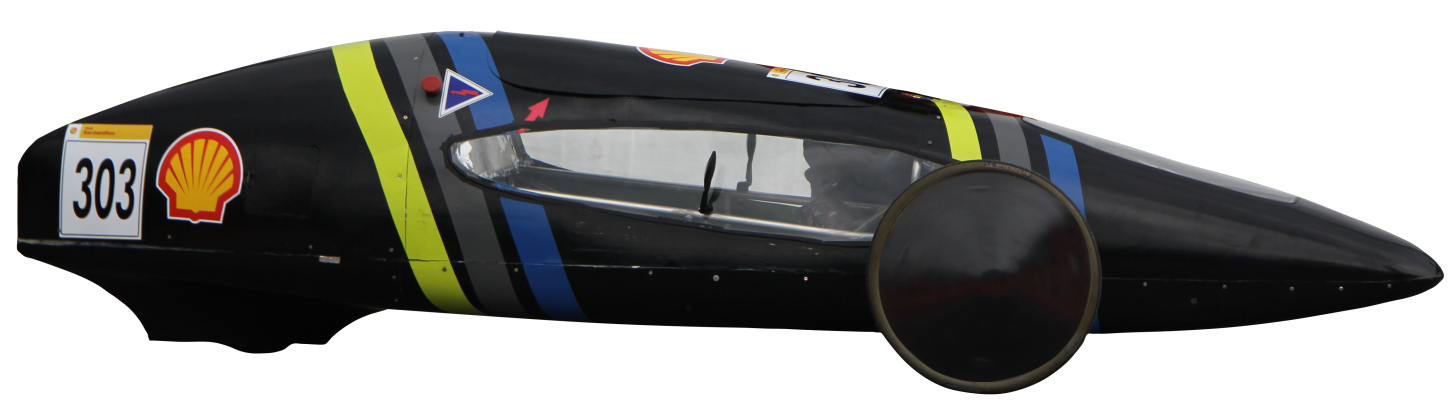
\includegraphics[angle=0, scale=0.8]{1_Introducao/Figuras/dt1.png}
    \caption{Battery electric prototype vehicle DT1}
    \label{fig1}
\end{figure}


